\documentclass[runningheads]{llncs}
\usepackage{packages}
\usepackage{statmacros}
\newcolumntype{C}[1]{>{\centering\arraybackslash}p{#1}}
\setlength{\textfloatsep}{10pt plus 1.0pt minus 2.0pt}
\renewcommand\theoremname{Teorema}

\begin{document}

\title{Clustering distribuito tramite MapReduce}

\author{Daniele Zago\inst{1} e Giovanni Toto\inst{2}}


\institute{Corso di laurea in Scienze Statistiche, matricola 1237310
\email{daniele.zago.1@studenti.unipd.it}\and
Corso di laurea in Scienze Statistiche, matricola 1242466
\email{giovanni.toto@studenti.unipd.it}}

\maketitle

\begin{abstract}
%Qui si scrive il riassunto del tema, del problema specifico affrontato, dell'approccio seguito e dei risultati principali.  
In questo lavoro si propone un'implementazione di alcuni algoritmi di \textit{clustering} secondo il modello \textit{MapReduce} di elaborazione parallela e distribuita.
Dopo una presentazione teorica degli algoritmi $k$-\textit{means}, \textit{fuzzy} $c$-\textit{means}, e dell'architettura \mr, si discutono le scelte effettuate nello sviluppo del software.
Si mostra inoltre l'implementazione in \mr\ dell'inizializzazione $k$\textit{-means}++, metodo che permette una selezione probabilistica dei centroidi prima dell'avvio degli algoritmi.
Infine, si effettuano alcune simulazioni degli algoritmi su un insieme di dati reali, per verificare il funzionamento del software e l'impatto delle diverse inizializzazioni sulla convergenza.
\keywords{\emph{clustering}   \and \km \and \km++ \and \fcm \and \textit{MapReduce}\and \textit{architettura distribuita}}
\end{abstract}

\section{Introduzione}
% Nell'introduzione si deve scrivere tutto e solo ci\`o che serve.
% - rendere esplicito qual \`e il messaggio che lo studente deve ``portarsi a casa''
% - esplicitare i motivi per cui il problema affrontato \`e significativo 
% - discutere \emph{efficacia} ed \emph{efficienza} dei metodi illustrati 
% Per significativit\`a si intende l'interesse
% teorico-scientifico o l'impatto industriale che avrebbe la soluzione
% del problema (o entrambi).  Per efficacia si intende la capacit\`a di un metodo di
% risolvere il problema; l'efficienza \`e relativa al costo
% computazionale necessario. Il messaggio da ``portare a casa'' \`e ci\`o  su cui bisogna concentrarsi anche nel resto della relazione. 
Nel \textit{data science} è di particolare rilevanza raggruppare elementi simili, in modo da identificare associazioni nei dati ed effettuare operazioni di aggregazione su di essi~\cite{tan2005}.
Per insiemi di dati di grandi dimensioni, a volte tali da non poter essere caricati in memoria, è necessario ricorrere ad architetture di calcolo distribuite per l'implementazione degli algoritmi.
Una possibile soluzione è \mr, un'architettura sviluppata inizialmente da \textit{Google} e successivamente implementata in \textit{Hadoop}, che applica la logica del \textit{divide et impera} per l'elaborazione parallela dei dati~\cite{lin}.
In questo lavoro viene proposta un'implementazione in \textit{Python 3.6} degli algoritmi \km\ e \fcm\ secondo il paradigma \mr, attraverso l'uso della libreria \textit{MrJob}~\cite{marin2020}.

\section{Base di partenza}\label{cap:base_di_partenza}
%La base di partenza \`e formata dai metodi documentati nei libri di
%testo.  Si eviti di trascrivere pari pari, si cerchi piuttosto di
%rielaborare i contenuti in modo da renderli \emph{coerenti} col resto
%della relazione; in particolare, si descrivano tutti e solo i metodi
%usati negli esperimenti e si eviti di parlare di quei metodi che poi
%non sono stati usati; ad esempio, se si conducono degli esperimenti
%con BM25F, si deve descrivere questo schema di pesatura in questa
%sezione. 
L'analisi dei gruppi (\textit{cluster analysis}) è un insieme di metodi che, in generale, suddividono l'insieme di dati $\mathcal{X}$ in sottoinsiemi i cui membri risultano \textit{simili} tra loro.
In base al dominio applicativo e allo specifico metodo di raggruppamento, è possibile scegliere in modo opportuno cosa si intende per \textit{similarità} tra elementi $x \in \mathcal{X}$.
Nello specifico, i metodi \km\ e \fcm\ interpretano i dati $x$ come vettori di uno spazio vettoriale $\mathcal{X} \subseteq \R^{p}$, sul quale è definita una funzione distanza $d(\cdot , \cdot)$.
% Solitamente, la similarità tra due elementi $x_i$ e $x_j$ si pone pari alla distanza euclidea $d(x_i, x_j) = \|x_i - x_j\|_2$, in quanto si può dimostrare che scegliendo questa distanza l'algoritmo \km\ converge {\color{red}(?)}.
La procedura di raggruppamento porta alla minimizzazione di una funzione obiettivo $\loss(\cdot )$, la cui specificazione dipende dalla funzione $d(\cdot , \cdot )$, dal numero di cluster $k$ ed, eventualmente, da ulteriori parametri -- il parametro $m$ nel metodo \fcm.

I metodi proposti sono esempi di due tipologie di \textit{clustering} differenti:
\km\ produce un raggruppamento esclusivo, in cui ogni elemento appartiene ad uno ed un solo \textit{cluster}; \fcm, invece porta ad un raggruppamento \textit{fuzzy}, nel quale ogni elemento appartiene con un certo peso (\emph{membership weight}) a ciascun gruppo.
L'obiettivo di entrambi i metodi è creare delle partizioni che minimizzino la similarità tra gli elementi appartenenti allo stesso gruppo.
Se da un lato \km\ impone una netta separazione, \fcm\ sfuma questo aspetto, in modo da poter gestire elementi non facilmente categorizzabili nei \textit{cluster} trovati.
Infine, i due metodi si dicono \emph{prototype based} poiché ogni cluster è rappresentato da un centroide\footnote{Un centroide è oggetto, calcolato in maniera differente in base all'algoritmo scelto, che rappresenta tutti gli elementi contenuti nel cluster ad esso associato.}.

Dal momento che i centroidi, e quindi i \textit{cluster}, riassumono l'informazione contenuta nel dataset, il loro utilizzo permette di catturare la struttura naturale dei dati.
La possibilità di aggregare i dati attraverso i gruppi permette inoltre di ridurre la dimensione del dataset~\cite{tan2005}.

\subsection*{Algoritmo \km}
L'algoritmo \km\ opera una partizione dello spazio $\mathcal{X}$ in insiemi $R_1, R_2, \ldots, R_k$, tali cioè che $R_j \cap R_i = \emptyset $ per $j \neq i$ e $ \bigcup_{j = 1}^k R_j = \mathcal{X} $.
Per fare ciò, si devono individuare i centroidi $c_1, c_2, \ldots, c_k$ che minimizzino la funzione obiettivo
\[
    \loss(c_1, \ldots, c_k) = \sum_{j=1}^{k} \sum_{x_i \in R_k} d(x_i, c_j)^2 ,
\]
che nel caso si scelga la norma euclidea hanno soluzione esplicita e pari a
\[
    c_j = \frac{1}{|R_j|}\sum_{x \in R_j} x,
\]
L'algoritmo di stima procede ad ogni iterazione assegnando a ciascun insieme i punti ad esso più vicini, ricalcolandone successivamente i centroidi. Alternando questi due passaggi fino a convergenza, è possibile ottenere un minimo locale della funzione $\loss(c_1, c_2, \ldots, c_k)$.

{\centering
\begin{algorithm}[H]
\caption{\km}
\begin{algorithmic}[1]
    \Require $c^{0}_1, c^{0}_2, \ldots, c^{0}_k$
    \item[]
    \While{$\max_j d(c_j^{l+1}, c_j^{l}) > \varepsilon$}
        \For{$j \in 1, \ldots, k$}
        \State $R^{l+1}_j \leftarrow \{x \in \mathcal{X} : \argmin_{h = 1, \ldots, k} d(x , c^{l}_h) = j \} $
        \EndFor
        \For{$j \in 1, \ldots, k$}
        \State $c_j^{l+1} \leftarrow \frac{1}{n_j}\sum_{x \in R_j^{l+1}} x $
        \EndFor
    \EndWhile
\end{algorithmic}
\end{algorithm}
}

\subsection*{Algoritmo \fcm}
L'algoritmo \fcm\ è un'estensione dell'algoritmo \km\ in cui ogni osservazione appartiene a tutti i cluster simultaneamente con diverso peso.
La procedura richiede la specificazione di un ulteriore parametro $m \geqslant 1$, detto \textit{grado di mescolamento}, che determina quanto risulteranno \emph{fuzzy} i \textit{cluster} prodotti dall'algoritmo.

Per tenere traccia del grado di appartenenza di ogni osservazione ai vari cluster, si definisce la matrice di appartenenza $U = \left( u_{ij} \right)$, il cui singolo elemento $u_{ij}$ è il peso con cui l'$i$-ma osservazione appartiene al $j$-mo cluster.
La matrice $U$ è vincolata ad essere una matrice stocastica, ovvero $u_{ij} \in [0,1]$ per $i = 1, \ldots, n$ e $j = 1, \ldots, k$ e per ogni osservazione, $\sum_{j=1}^{k} u_{ij} = 1$.

L'algoritmo di stima minimizza la funzione obiettivo
\[
    \loss(c_1, \ldots, c_k) = \sum_{j=1}^{k} \sum_{i=1}^{n} u_{ij}^{m}d(x_i, c_j)^2 ,
\]
che nel caso della norma euclidea ha soluzione esplicita
\[
    c_j =\frac{ \sum_{i=1}^{n} u_{ij}^{m} x_i}{\sum_{i=1}^{n} u_{ij}^{m}}.
\]
Si noti che l'algoritmo \km\ è un caso particolare del \fcm, che si può ottenere fissando $m=1$ e modificando i vincoli di $U$ in modo tale che $u_{ij} \in \{0,1\}$, $i = 1, \ldots, n$, $j = 1, \ldots, k$.

Ad ogni iterazione, il procedimento di stima costruisce la matrice di appartenenza sulla base dei dati e dei centroidi correnti, per poi aggiornare i centroidi utilizzando la soluzione esplicita del problema di minimo.
Come nel caso dell'algoritmo \km, i due passaggi vengono alternati fino a convergenza ad un minimo locale della funzione $\loss(c_1, c_2, \ldots, c_k)$.

{\centering
\begin{minipage}{\textwidth}
\begin{algorithm}[H]
\caption{\fcm}
\begin{algorithmic}[1]
    \Require $c^{0}_1, c^{0}_2, \ldots, c^{0}_k$, $m$
    \item[]
    \While{$\max_j d(c_j^{l+1}, c_j^{l}) > \varepsilon$}
        \For{$i \in 1, \ldots, n$}
            \For{$j \in 1, \ldots, k$}
            \State $u_{ij} \leftarrow \left(\sum_{h=1}^{k} \Big(\frac{d(x_i, c^{l}_j)}{d(x_i, c^{l}_h)}\Big)^{\frac{2}{m-1}}\right)^{-1} $
            \EndFor
        \EndFor
        \For{$j \in 1, \ldots, k$}
            \State $c^{l+1}_j \leftarrow \dfrac{\sum_{i=1}^{n} u_{ij}^{m}x_i}{\sum_{i=1}^{n} u_{ij}^{m}}$
        \EndFor
    \EndWhile
\end{algorithmic}
\end{algorithm}
\end{minipage}
\par\bigskip
}

Non sono presenti basi teoriche che identifichino un valore ottimale per $m$ o giustifichino la scelta di un valore rispetto ad un altro ma, per la maggior parte degli insiemi di dati, l'evidenza empirica suggerisce che $m$ sia compreso tra $1.5$ e $30$.

In generale, se $m \rightarrow 1$, si ha una forte distinzione tra i gruppi (\textit{hard clustering}), mentre se $m \rightarrow +\infty$ ogni elemento della matrice $U$ tenderà a $1/k$ (\textit{fuzziest state}, in cui ogni osservazione appartiene in egual misura a tutti i cluster).

\subsection*{Inizializzazione dei centroidi}
Sia l'algoritmo \km\ sia l'algoritmo \fcm\ richiedono come input una lista di punti nello spazio $\mathcal{X}$, che vengono utilizzati come i centroidi iniziali.
Il numero di punti forniti definisce il numero $k$ di centroidi di riferimento, ma esso può diminuire poiché un cluster viene eliminato se nessun punto viene associato ad esso durante una qualunque iterazione.
Il processo di selezione di questi $k$ punti è detto \emph{inizializzazione dei centroidi} e può essere effettuato in diversi modi. Di seguito sono riportate le tre inizializzazioni considerate nel progetto.

\paragraph{Inizializzazione casuale}
Si selezionano casualmente $k$ osservazioni dal dataset da utilizzare come centroidi iniziali. È l'alternativa più intuitiva e semplice da implementare, ma anche una strategia sub-ottimale dal momento che la selezione totalmente casuale può influenzare sia la qualità della previsione sia la velocità di convergenza.


\paragraph{Inizializzazione a step}
In un primo momento, viene identificato il range dei possibili valori di ogni variabile disponibile, definito come
\[
    (x^{min}_h,x^{max}_h)= \big(\min\{{x_{1h}, \ldots, x_{nh}}\}, \max\{{x_{1h}, \ldots, x_{nh}}\} \big), \quad h=1, \ldots, p
\]
dove $x_{ih}$ è il valore che assume la $h$-ma variabile nell'$i$-ma osservazione. Quindi, per ogni variabile, viene calcolato uno step $s_h=\frac{x^{max}_h-x^{min}_h}{k}$ che permette di ottenere i centroidi nel seguente modo
\[
    c_j =
    \begin{bmatrix}
    x^{min}_1\\
    \vdots\\
    x^{min}_p\\
    \end{bmatrix}
    +
    \begin{bmatrix}
    s_1\\
    \vdots\\
    s_p\\
    \end{bmatrix}
    \times (j-1)
\]
I centroidi così selezionati coprono l'intero spazio $\mathcal{X}$, ma il risultato finale è fortemente influenzato da valori anomali e non tiene conto della distribuzione dei dati.


\paragraph{Inizializzazione \texttt{++}}
Permette di disperdere i centroidi iniziali nello spazio $\mathcal{X}$, tenendo tuttavia conto della distribuzione dei dati. Il primo centroide viene selezionato casualmente, mentre la selezione del $j$-esimo centroide è legata dai $j-1$ centroidi già scelti~\cite{stetco2015}; in particolare, la probabilità che il punto $x$ venga scelto come centroide è pari a 
\[
    \frac{ d(x,\mathcal{R})^{p}}{\sum_{x' \in \mathcal{X}} d(x',\mathcal{R})^{p}},
\]
dove $\mathcal{R}$ è l'insieme dei centrodi già selezionati, $d(x,\mathcal{R})^{p}$ è la distanza tra il punto $x$ e il centroide in $\mathcal{R}$ più vicino ad esso, $p>0$ è un parametro che controlla quanto distribuire i centroidi nello spazio $\mathcal{X}$.

Se $p \rightarrow 0$, la selezione sarà del tutto casuale; al contrario, se $p \rightarrow \infty$, verranno selezionati gli outlier. Assumendo che dei buoni centroidi si distribuiscano in tutto lo spazio, la scelta di $p$ deve essere una via di mezzo tra i due estremi. In generale, per $p \in (0.1,1.3)$, l'algoritmo \fcm\ (o \km) ottiene risultati molto volatili e prestazioni simili a quelli con un'inizializzazione casuale, mentre per $p$ maggiori si ottengono risultati meno volatili e sono necessarie meno iterazioni per raggiungere la convergenza \cite{stetco2015}.
Solitamente, con inizializzazione \texttt{++} ci si riferisce al caso in cui $p = 2$.

\subsection*{MapReduce}
MapReduce è un framework per la creazione di applicazioni in grado di elaborare grandi quantità di dati in parallelo. L'architettura si fonda sul concetto di programmazione funzionale, in cui i dati sono passati tra le funzioni come parametri, e sull'idea di poter dividere l'algoritmo in sotto-processi indipendenti tra loro.
Più nello specifico, ogni funzione riceve in input i dati nella forma $\langle \textit{chiave, valore} \rangle$ e, dopo una serie di processi intermedi, ritorna come output un'altra coppia $\langle \textit{chiave, valore} \rangle $.

Esistono diversi tipi di processi intermedi ma i due fondamentali, che devono sempre essere definiti, sono:
\begin{itemize}
    \item[--] funzione \emph{map}: riceve in input un elemento nella forma $\langle$\emph{i, i-ma oss.}$\rangle$ e crea come output zero o più coppie $\langle$\emph{chiave, valore}$\rangle$\\[-0.2cm]
    \item[--] funzione \emph{reduce}: per ogni chiave, elabora i valori ad essa associati e crea come output zero o più coppie $\langle$\emph{chiave, valore}$\rangle$
\end{itemize}

Quindi, in un primo momento l'elaborazione dei dati produce un insieme di coppie $\langle \textit{chiave, valore} \rangle $.
Successivamente, valori associati ad una stessa chiave sono raggruppati sotto forma di iteratori e su di essi vengono effettuate delle operazioni di aggregazione.
Se necessario, è possibile inserire ulteriori processi intermedi che permettono di implementare algoritmi più complessi.

Una peculiarità di MapReduce è che viene nascosta al programmatore la complessità derivante dalla parallelizzazione e si fornisce un'astrazione che permette di trascurare i dettagli system-level\footnote{Esempi di dettagli system-level sono la gestione del trasferimento di dati tra diverse macchine o la gestione del fallimento di processi intermedi.}, dal momento che è \emph{MapReduce} stesso ad occuparsene.
Quindi, il programmatore non deve occuparsi di come le computazioni necessarie vengono svolte, ma deve solo definire cosa queste ultime devono fare.

\section{Metodi proposti}
Si propone un implementazione in \textit{Python} degli algoritmi \km\ e \fcm\ secondo il paradigma \mr, attraverso l'utilizzo della libreria \textit{mrjob}~\cite{marin2020}. In entrambi i casi, poiché questa libreria impone l'esecuzione di un singolo \textit{job} per istanza di \mr, è stato necessario utilizzare uno script che chiamasse ripetutamente gli algoritmi fino a convergenza. Questa soluzione non è ottimale, in quanto aggiunge un costo computazionale significativo dato dalla ripetuta inizializzazione e distruzione degli oggetti che gestiscono la parallelizzazione.
I due algoritmi sono stati implementati seguendo le specifiche di \cite{zhao2009} e \cite{ludwig2015}. Successivamente, si propone anche un'implementazione in \mr\ delle inizializzazioni a step, random e ++, quest'ultima secondo le specifiche descritte in~\cite{bodoia}. Poiché nell'articolo di riferimento è assente, viene infine proposta una dimostrazione della correttezza dell'algoritmo.
\subsection*{\mr: \km}
L'algoritmo \emph{PKMeans}, proposto in \cite{zhao2009}, nella sua versione più semplice necessita di un singolo \textit{job} \textit{map} e \textit{reduce}.

La funzione \emph{map} esegue la procedura di assegnazione di ogni osservazione al centroide più vicino, mentre la funzione \emph{reduce} aggiorna i centroidi sulla base degli insiemi appena calcolati. In particolare, la funzione \emph{reduce}, che riceve come chiave l'indice del cluster considerato e come valore la lista dei punti ad esso assegnati, calcola semplicemente la media dei punti ricevuti in input. 

\begin{minipage}[t]{0.48\textwidth}
\begin{algorithm}[H]
\caption{\km\ \textit{map}}
\begin{algorithmic}[1]
    \setstretch{1.15}
    \Require $c_1, c_2, \ldots, c_k, x_i$
    \Ensure $\langle j, x_i \rangle $
    \State $j = \argmin_{h = 1, \ldots, k} d(x_i, c_h)$
    \State \Return $\langle j, x_i \rangle$
\end{algorithmic}
\end{algorithm}
\end{minipage}%
\hspace{\fill}
\begin{minipage}[t]{0.48\textwidth}
\begin{algorithm}[H]
\caption{\km\ \textit{reduce}}
\begin{algorithmic}[1]
    \setstretch{1.15}
    \Require $\langle j, R_j \rangle$
    \Ensure $\langle j, c_j \rangle$
    \State $c_j \leftarrow \frac{1}{|R_j|}\sum_{x \in R_j} x$
    \State \Return $\langle j, c_j \rangle $
\end{algorithmic}
\end{algorithm}
\end{minipage}


\subsection*{\mr: \fcm}
L'algoritmo \textit{MR-FCM}, proposto in \cite{ludwig2015}, necessita di due \textit{job}, ciascuno formato da una funzione \textit{map} e una funzione \textit{reduce}: il primo costruisce la matrice di appartenenza sulla base dei centroidi, mentre il secondo aggiorna questi ultimi con il risultato del primo \textit{job}. È possibile tuttavia evitare l'esecuzione di due istanze di \mr\ ad ogni passo dell'algoritmo, se si sfrutta la struttura delle formule di aggiornamento.\\
% Dal momento che il criterio di arresto considerato non richiede la matrice di appartenenza e quindi non è necessario calcolare la matrice ad ogni iterazione, si propone un nuovo algoritmo, formato da un singolo \textit{job} di \mr, che aggiorna direttamente i centroidi senza dover creare prima l'intera matrice di appartenenza. 

Considerando la funzione di aggiornamento del singolo elemento $u_{ij}$ di $U$, si può notare che essa dipende solo dai centroidi precedenti e dall'$i$-mo punto del dataset:
\[
    u_{ij} = \left(\sum_{h=1}^{k} \Big(\frac{d_{ij}}{d_{ih}}\Big)^{\frac{2}{m-1}}\right)^{-1}.
\]
Allo stesso modo, si osserva che l'aggiornamento del $j$-esimo centroide,
\[
    c_j = \frac{\sum_{i=1}^{n} u_{ij}^{m}x_i}{\sum_{i=1}^{n} u_{ij}^{m}},
\]
avviene unicamente attraverso le coppie di valori $\{(u_{ij}^{m}x_i, u_{ij}^{m})\}_{i=1}^n$, cioè utilizzando la sola $j$-esima colonna di $U$. Alla luce di queste osservazioni, si propone un'implementazione con un singolo \textit{job}, che aggiorna i centroidi evitando di dover ripetutamente salvare su disco l'intera matrice di appartenenza.
La funzione \textit{map} riceve in input l'$i$-mo punto del dataset, calcola l'$i$-ma riga di $U$ e ritorna $k$ coppie $\langle j, (u_{ij}^{m} x_i, u_{ij}^{m}) \rangle $. In questo modo, la funzione \textit{reduce} riceve in input le coppie $\left< j, [(u_{1j}^{m} x_1, u_{1j}^{m}), \ldots, (u_{nj}^{m}x_n, u_{nj}^{m})]\right>$, che sono sufficienti per aggiornare il $j$-esimo centroide.
% Ne consegue che l'$i$-mo addendo di entrambe le sommatorie presenti nella formula di aggiornamento dei centroidi è funzione dei centroidi,  dell'$i$-mo punto e del grado di mescolamento:
% Inoltre, data un singola osservazione, è possibile calcolare la riga corrispondente di $U$ e, per calcolare il $j$-mo centroide aggiornato, sono necessari tutte i punti e la $j$-ma colonna di $U$.



\begin{minipage}[t]{0.48\textwidth}
\begin{algorithm}[H]
\caption{\fcm\ \textit{map}}
\begin{algorithmic}[1]
    \setstretch{1.15}
    \Require $c_1, c_2, \ldots, c_k, x_i$
    \Ensure $\langle j, (u_{ij}^{m} x_i, u_{ij}^{m}) \rangle $, $j = 1, \ldots, k$
    \For{$j = 1, \ldots, k$}
        \State $d_{ij} \leftarrow d(x_i, c_j)$
    \EndFor
    \For{$j = 1, \ldots, k$}
        \State $u_{ij} \leftarrow \left(\sum_{h=1}^{k} \Big(\frac{d_{ij}}{d_{ih}}\Big)^{\frac{2}{m-1}}\right)^{-1} $ 
    \EndFor
    \State \Return $\langle j, (u_{ij}^{m}x_i, u_{ij}^{m}) \rangle $, $j = 1, \ldots, k$
\end{algorithmic}
\end{algorithm}
\end{minipage}
\hspace{\fill}
\begin{minipage}[t]{0.48\textwidth}
\begin{algorithm}[H]
\caption{\fcm\ \textit{reduce}}
\begin{algorithmic}[1]
    \setstretch{1.15}
    \Require $\langle j, [(u_{1j}^{m} x_1, u_{1j}^{m}), \ldots, (u_{nj}^{m}x_n, u_{nj}^{m})]\rangle $
    \Ensure $\langle j, c_j \rangle$
    \State $c_j \leftarrow \frac{\sum_{i=1}^{n} u_{ij}^{m}x_i}{\sum_{i=1}^{n} u_{ij}^{m}} $
    \State\Return $\langle j, c_j \rangle $
\end{algorithmic}
\end{algorithm}
\end{minipage}


\subsection*{\mr: inizializzazione a step}
L'inizializzazione a step necessita di un singolo job: la funzione \emph{map} legge le osservazioni e le converte in vettori, mentre la funzione \emph{reduce} calcola lo step per ogni feature e calcola $k$ centroidi con la formula esposta in precedenza. A livello pratico, questa implementazione velocizza esclusivamente la lettura della osservazioni da file di testo.
\begin{minipage}[t]{0.48\textwidth}
\begin{algorithm}[H]
\caption{Inizializzazione a step \textit{map}}
\begin{algorithmic}[1]
    \setstretch{1.15}
    \Require $x_i$
    \Ensure $\langle  \text{\_}, x_i \rangle$
    \State \Return $\langle  \text{\_}, x_i \rangle$
\end{algorithmic}
\end{algorithm}
\end{minipage}%
\hspace{\fill}
\begin{minipage}[t]{0.48\textwidth}
\begin{algorithm}[H]
\caption{Inizializzazione a step \textit{reduce}}
\begin{algorithmic}[1]
    \setstretch{1.15}
    \Require $\langle  \text{\_}, [x_1, \ldots, x_n] \rangle$
    \Ensure $\langle j, c_j \rangle$, $j = 1, \ldots, k$
    \For{$h = 1, \ldots, p$}
        \State $x^{min}_h = \min\{{x_{1h}, \ldots, x_{nh}}\}$
        \State $x^{max}_h = \max\{{x_{1h}, \ldots, x_{nh}}\}$
    \EndFor
    \State $s = \frac{1}{j}(x^{max} - x^{min})$
    \For{j = 1, \ldots, k}
        \State $c_j = x^{min}+ s(j-1)$
    \EndFor
    \State \Return $\langle j, c_j \rangle$, $j = 1, \ldots, k$
\end{algorithmic}
\end{algorithm}
\end{minipage}


\subsection*{\mr: inizializzazione ++}
Poiché l'inizializzazione ++ necessita di campionare probabilisticamente i dati sulla base dei centroidi precedentemente scelti, la sua implementazione in \mr\ è leggermente più complicata. In particolare, è stata utilizzata la procedura suggerita in~\cite{bodoia}, che confronta i dati a coppie: per ogni coppia $\left<x_1, d(x_1, \mathcal{R})^{p}\right>$ e $\left< x_2 , d(x_2, \mathcal{R})^{p}  \right>$, la funzione ritorna $\left<z,  d(x_1, \mathcal{R})^{p} + d(x_2, \mathcal{R})^{p}\right>$ dove
\[
    z = \begin{cases}
        x_1 & \text{con probabilità }\ \frac{d(x_1, \mathcal{R})^{p}}{d(x_1, \mathcal{R})^{p} + d(x_2, \mathcal{R})^{p}}\\[.2cm]
        x_2 & \text{con probabilità }\ 1 - \frac{d(x_1, \mathcal{R})^{p}}{d(x_1, \mathcal{R})^{p} + d(x_2, \mathcal{R})^{p}}\\
    \end{cases}.
\]
La coppia così ottenuta viene poi utilizzata per il confronto con la successiva $\left< x_3 , d(x_3, \mathcal{R})^{p} \right>$ e si ripete la procedura fino all'ultimo elemento del dataset. L'elemento $x_j$ selezionato al termine dell'iterazione viene aggiunto all'insieme $\mathcal{R}$ e si ripete l'algoritmo fino alla selezione di $k$ centroidi.

\begin{theorem}
    L'algoritmo sopra descritto seleziona un qualunque punto $x_j$ con probabilità pari a
    \[
        P(x_j |\mathcal{R})= \frac{d(x_j, \mathcal{R})^{p}}{\sum_{i=1}^{n} d(x_i, \mathcal{R})^{p}}.
    \]
\end{theorem}
\begin{proof}
    Si consideri il primo elemento $x_1$: affinché venga selezionato al termine dell'algoritmo, è necessario che venga selezionato ad ogni confronto a coppie e ciò avviene con probabilità
    \[
        \begin{aligned}
            P(x_1|\mathcal{R}) & = \frac{d(x_1, \mathcal{R})^{p}}{d(x_1, \mathcal{R})^{p} + d(x_2, \mathcal{R})^{p}} \times  \frac{d(x_1, \mathcal{R})^{p} + d(x_2, \mathcal{R})^{p}}{d(x_1, \mathcal{R})^{p} + d(x_2, \mathcal{R})^{p} + d(x_3, \mathcal{R})^{p}} \times  \cdots \times   \frac{\sum_{i = 2}^n d(x_i, \mathcal{R})^{p} }{\sum_{i = 1}^n d(x_i, \mathcal{R})^{p}}\\[.1cm]
                               &= \frac{d(x_1, \mathcal{R})^{p}}{\sum_{i=1}^{n} d(x_i, \mathcal{R})^{p}}. 
        \end{aligned}
    \]
    Sia ora un qualunque altro punto $x_j$: perché sia selezionato, è necessario che venga scelto al confronto con il $(j-1)$-esimo punto e per tutti gli $n-j-1$ confronti successivi. Ciò avviene con probabilità
    \[
        \begin{aligned}
            P(x_j|\mathcal{R})^{p} &= \frac{d(x_j, \mathcal{R})^{p}}{\sum_{i=1}^{j} d(x_i, \mathcal{R})^{p}} \times \frac{\sum_{i=1}^{j}d(x_i, \mathcal{R})^{p} }{\sum_{i=1}^{j+1}d(x_i, \mathcal{R})^{p}} \times \cdots \times \frac{\sum_{i = 2}^n d(x_i, \mathcal{R})^{p} }{\sum_{i = 1}^n d(x_i, \mathcal{R})^{p}}\\[.1cm]
            &= \frac{d(x_j, \mathcal{R})^{p}}{\sum_{i=1}^{n} d(x_i, \mathcal{R})^{p}}. 
        \end{aligned}
    \]
\end{proof}
La versione \mr\ dell'algoritmo è implementata nel modo seguente:

\begin{minipage}[t]{0.48\textwidth}
\begin{algorithm}[H]
    \caption{\textit{Inizializzazione ++ map}}
\begin{algorithmic}[1]
    \setstretch{1.15}
    \Require $\mathcal{R}, x_i$
    \Ensure $\langle x_i, D_{x_i}  \rangle $
    \State $D_{x_i} \leftarrow \min_{c \in \mathcal{R}} d(x_i, c)^p$
    \State\Return $\langle \text{\_}, (x_i, D_{x_i})\rangle $
\end{algorithmic}
\end{algorithm}
\end{minipage}
\vspace{\fill}
\begin{minipage}[t]{0.48\textwidth}
\begin{algorithm}[H]
    \caption{\textit{Inizializzazione ++ reduce}}
\begin{algorithmic}[1]
    \setstretch{1.15}
    \Require $\langle  \text{\_}, (x_1, D_{x_1}), \ldots,  (x_n, D_{x_n})\rangle$
    \Ensure $\langle c, D_c \rangle $
    \State $z \leftarrow x_1$
    \State $D_z \leftarrow D_{x_1}$
    \For{$i=2, \ldots, n$}
    \State \textbf{con probabilità }$D_z / (D_z + D_{x_i}):$ 
    \State \hspace*{0.5cm} $D_z \leftarrow D_z + D_{x_i}$
    \State \textbf{altrimenti} :
    \State \hspace*{0.5cm} $z \leftarrow x_i$
    \State \hspace*{0.5cm} $D_z \leftarrow D_z + D_{x_i}$
    \EndFor
    \State\Return $\langle z, D_z \rangle $
\end{algorithmic}
\end{algorithm}
\end{minipage}

\subsection*{\mr: inizializzazione random}
È immediato verificare che, ponendo $p=0$ nell'inizializzazione ++, si ottiene una probabilità di selezione uniforme
\[
    P(x_j | \mathcal{R}) = \begin{cases}
        0 & \text{se } x_j \in \mathcal{R}\\[.15cm]
        \dfrac{1}{n - |\mathcal{R}|} &\text{se } x_j \not\in \mathcal{R}
    \end{cases},
\]
per cui lo stesso algoritmo utilizzato per l'inizializzazione ++ può essere impiegato anche per l'inizializzazione random.

Un'alternativa più efficiente potrebbe sfruttare il fatto che \mr\ preveda la suddivisione in modo non deterministico dell'insieme di dati, per la procedura di \textit{map}. Di conseguenza, il \textit{job} potrebbe semplicemente ritornare $k$ punti e scartare i successivi per ottenere un campione casuale di elementi. Tuttavia, dopo qualche verifica, sembra che la libreria \textit{mrjob} effettui una suddivisione pseudo-casuale solamente per taglie di dati molto grandi, per cui si è preferito procedere con la prima opzione.

\section{Esperimenti}\label{cap:esperimenti}
In conclusione, sono state svolte alcune prove empiriche degli algoritmi proposti su un dataset reale, per verificare la scalabilità dell'implementazione e il costo computazionale.
L'interesse è confrontare la velocità di convergenza degli algoritmi \km\ e \fcm\ al variare del numero $k$ di cluster e del parametro di mescolamento $m$, oltre che valutare l'effetto delle diverse inizializzazioni discusse in precedenza.

L'insieme di dati considerato consiste di $n = 115473$ osservazioni e $p = 52$ variabili esplicative continue, con le unità raggruppate in $c = 5$ classi note. 
Il dataset è stato ottenuto in seguito al preprocessamento dei dati di un esame pratico del corso di ``Analisi dei Dati'', della Laurea Magistrale in Scienze Statistiche.
Poiché la numerosità delle classi risulta molto sbilanciata, con $3$ di esse che raccolgono il 90\% delle osservazioni, ci si aspetta che gli algoritmi difficilmente riescano ad identificare più di quattro classi.
Per questo motivo, si è deciso di effettuare i test degli algoritmi per $k = 3,4,5$.
Per le simulazioni, oltre al dataset originale sono stati estratti tre sottoinsiemi di osservazioni, di dimensione rispettivamente $n_1 = 15000$, $n_2 = 30000$ e $n_3 = 70000$, in modo da valutare la scalabilità degli algoritmi all'aumentare della taglia dei dati. Tutte le simulazioni sono state eseguite su un calcolatore con sistema operativo \textit{Lubuntu 19.04} e processore \textit{Intel Core i7-8700 CPU @3.20GHz} con 12 CPU.
In Figura~\ref{fig:results} sono riportati i risultati delle esecuzioni per i diversi sottoinsiemi di dati: l'algoritmo è stato eseguito 5 volte per ciascuna combinazione di iperparametri e inizializzazioni ed è stata riportata la media del numero di iterazioni necessarie per la convergenza.
Per l'inizializzazione ++ è stato scelto $p=2$, che è il valore più comunemente utilizzato in letteratura.
Tutti gli algoritmi sono stati terminati anticipatamente nel caso la convergenza non fosse stata raggiunta dopo 50 iterazioni.

\begin{center}
    % \centering
    % trim l b r u
    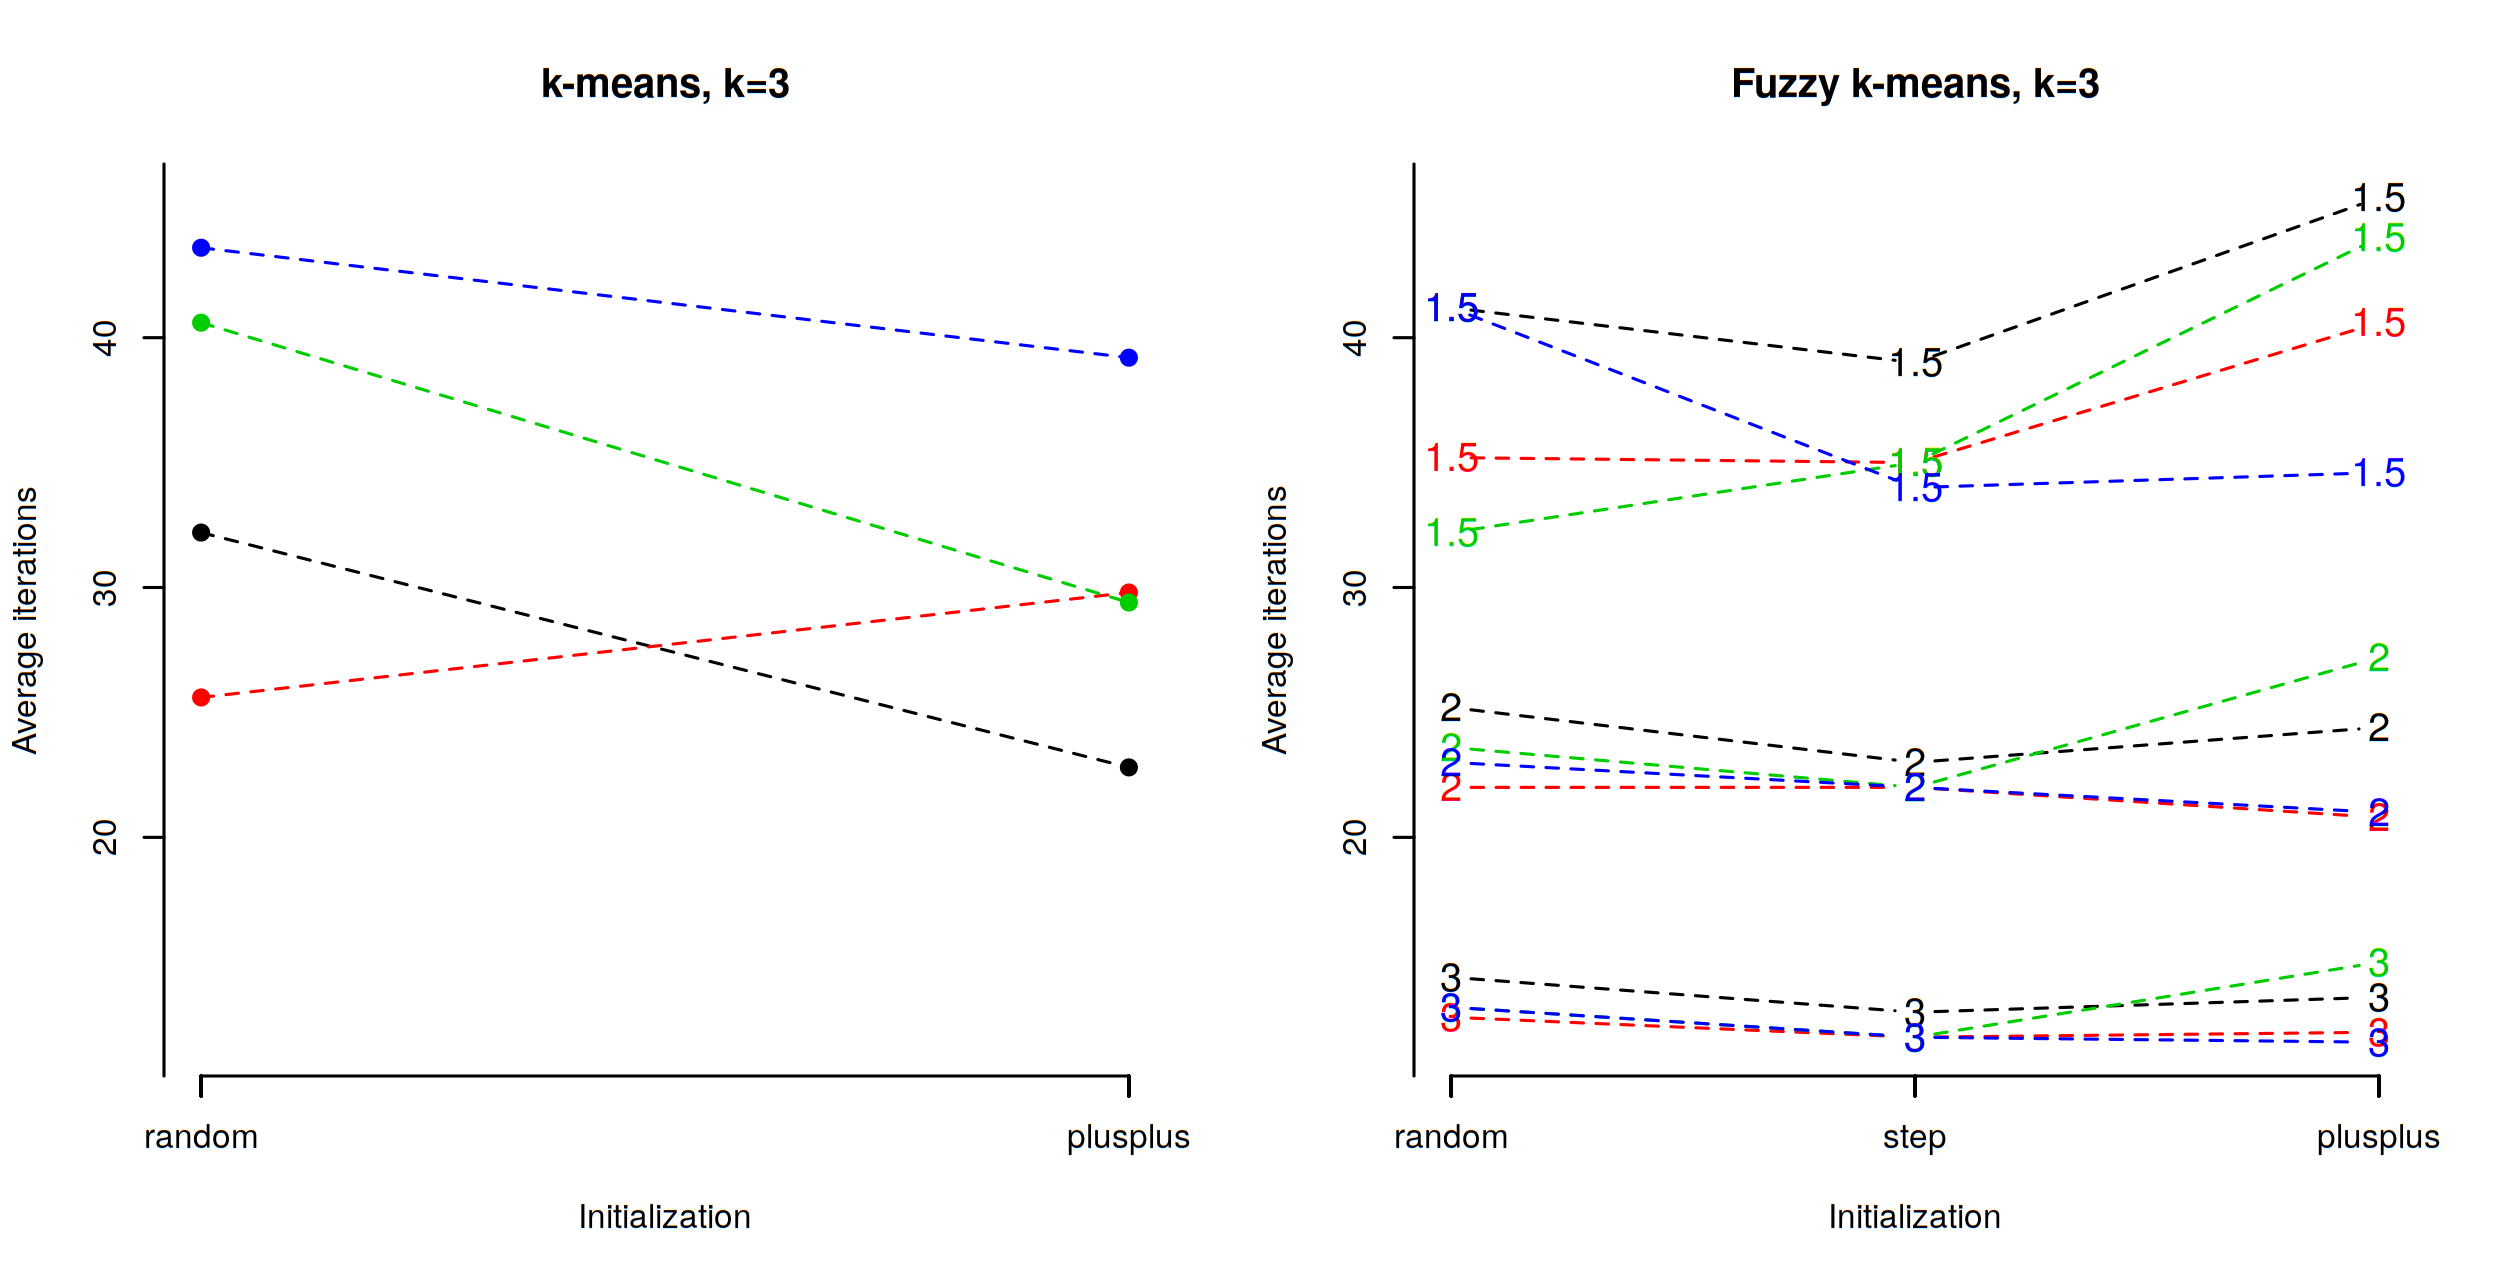
\includegraphics[width=0.94\textwidth]{figures/clust-3.png}
    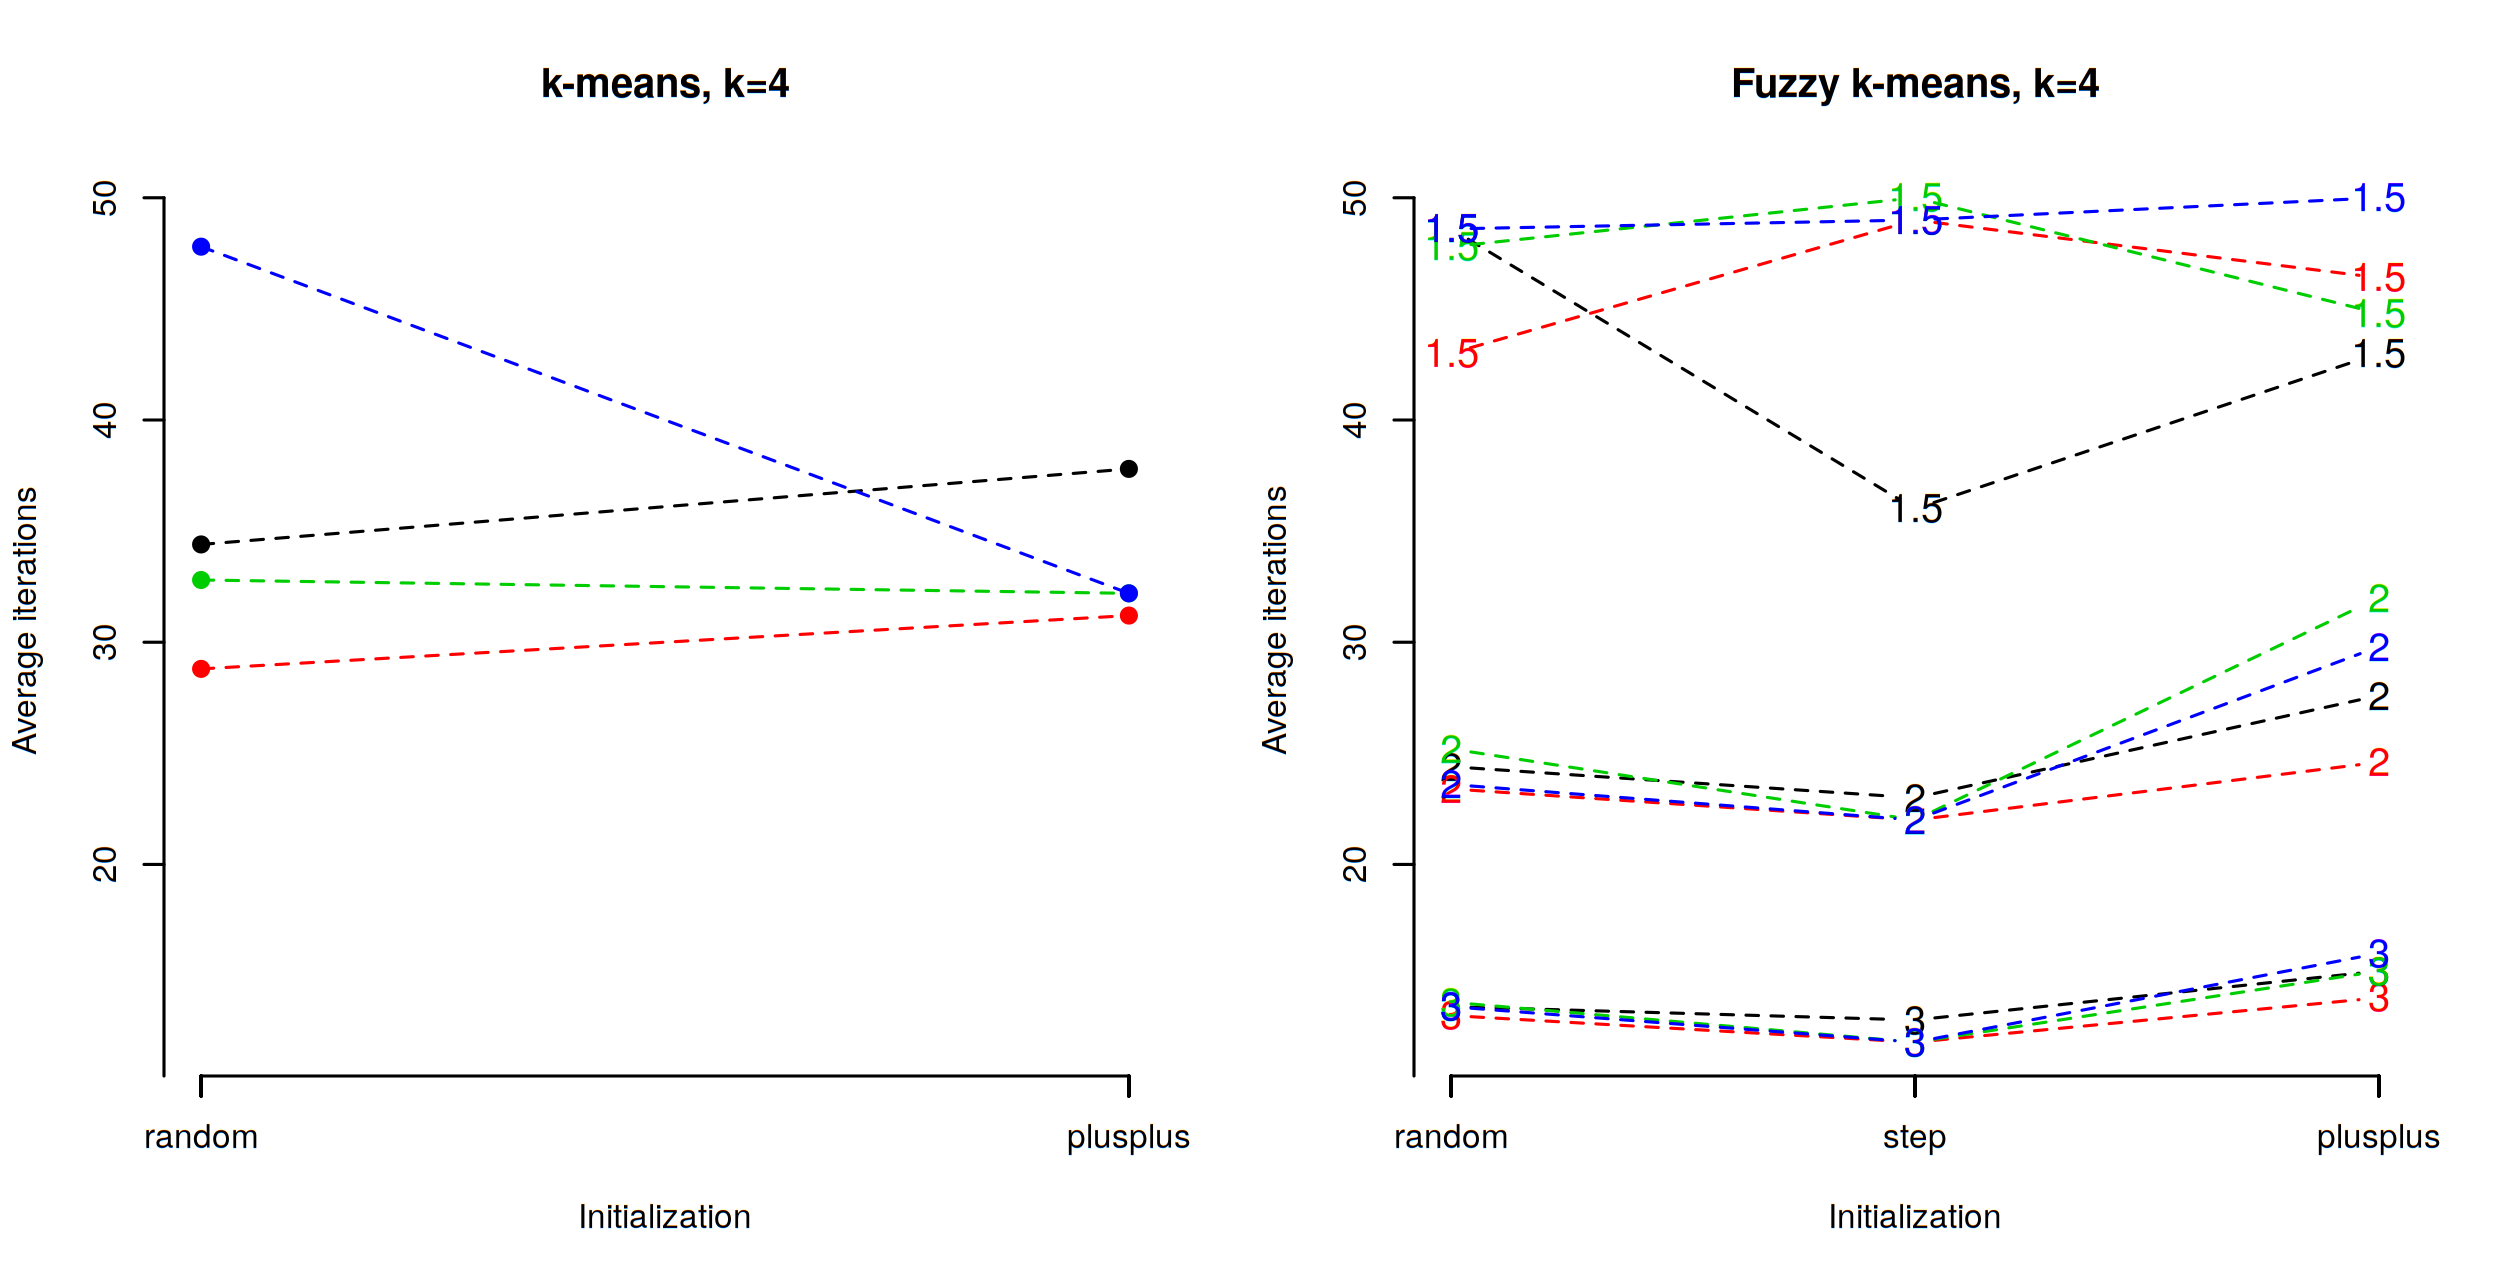
\includegraphics[width=0.94\textwidth]{figures/clust-4.png}
    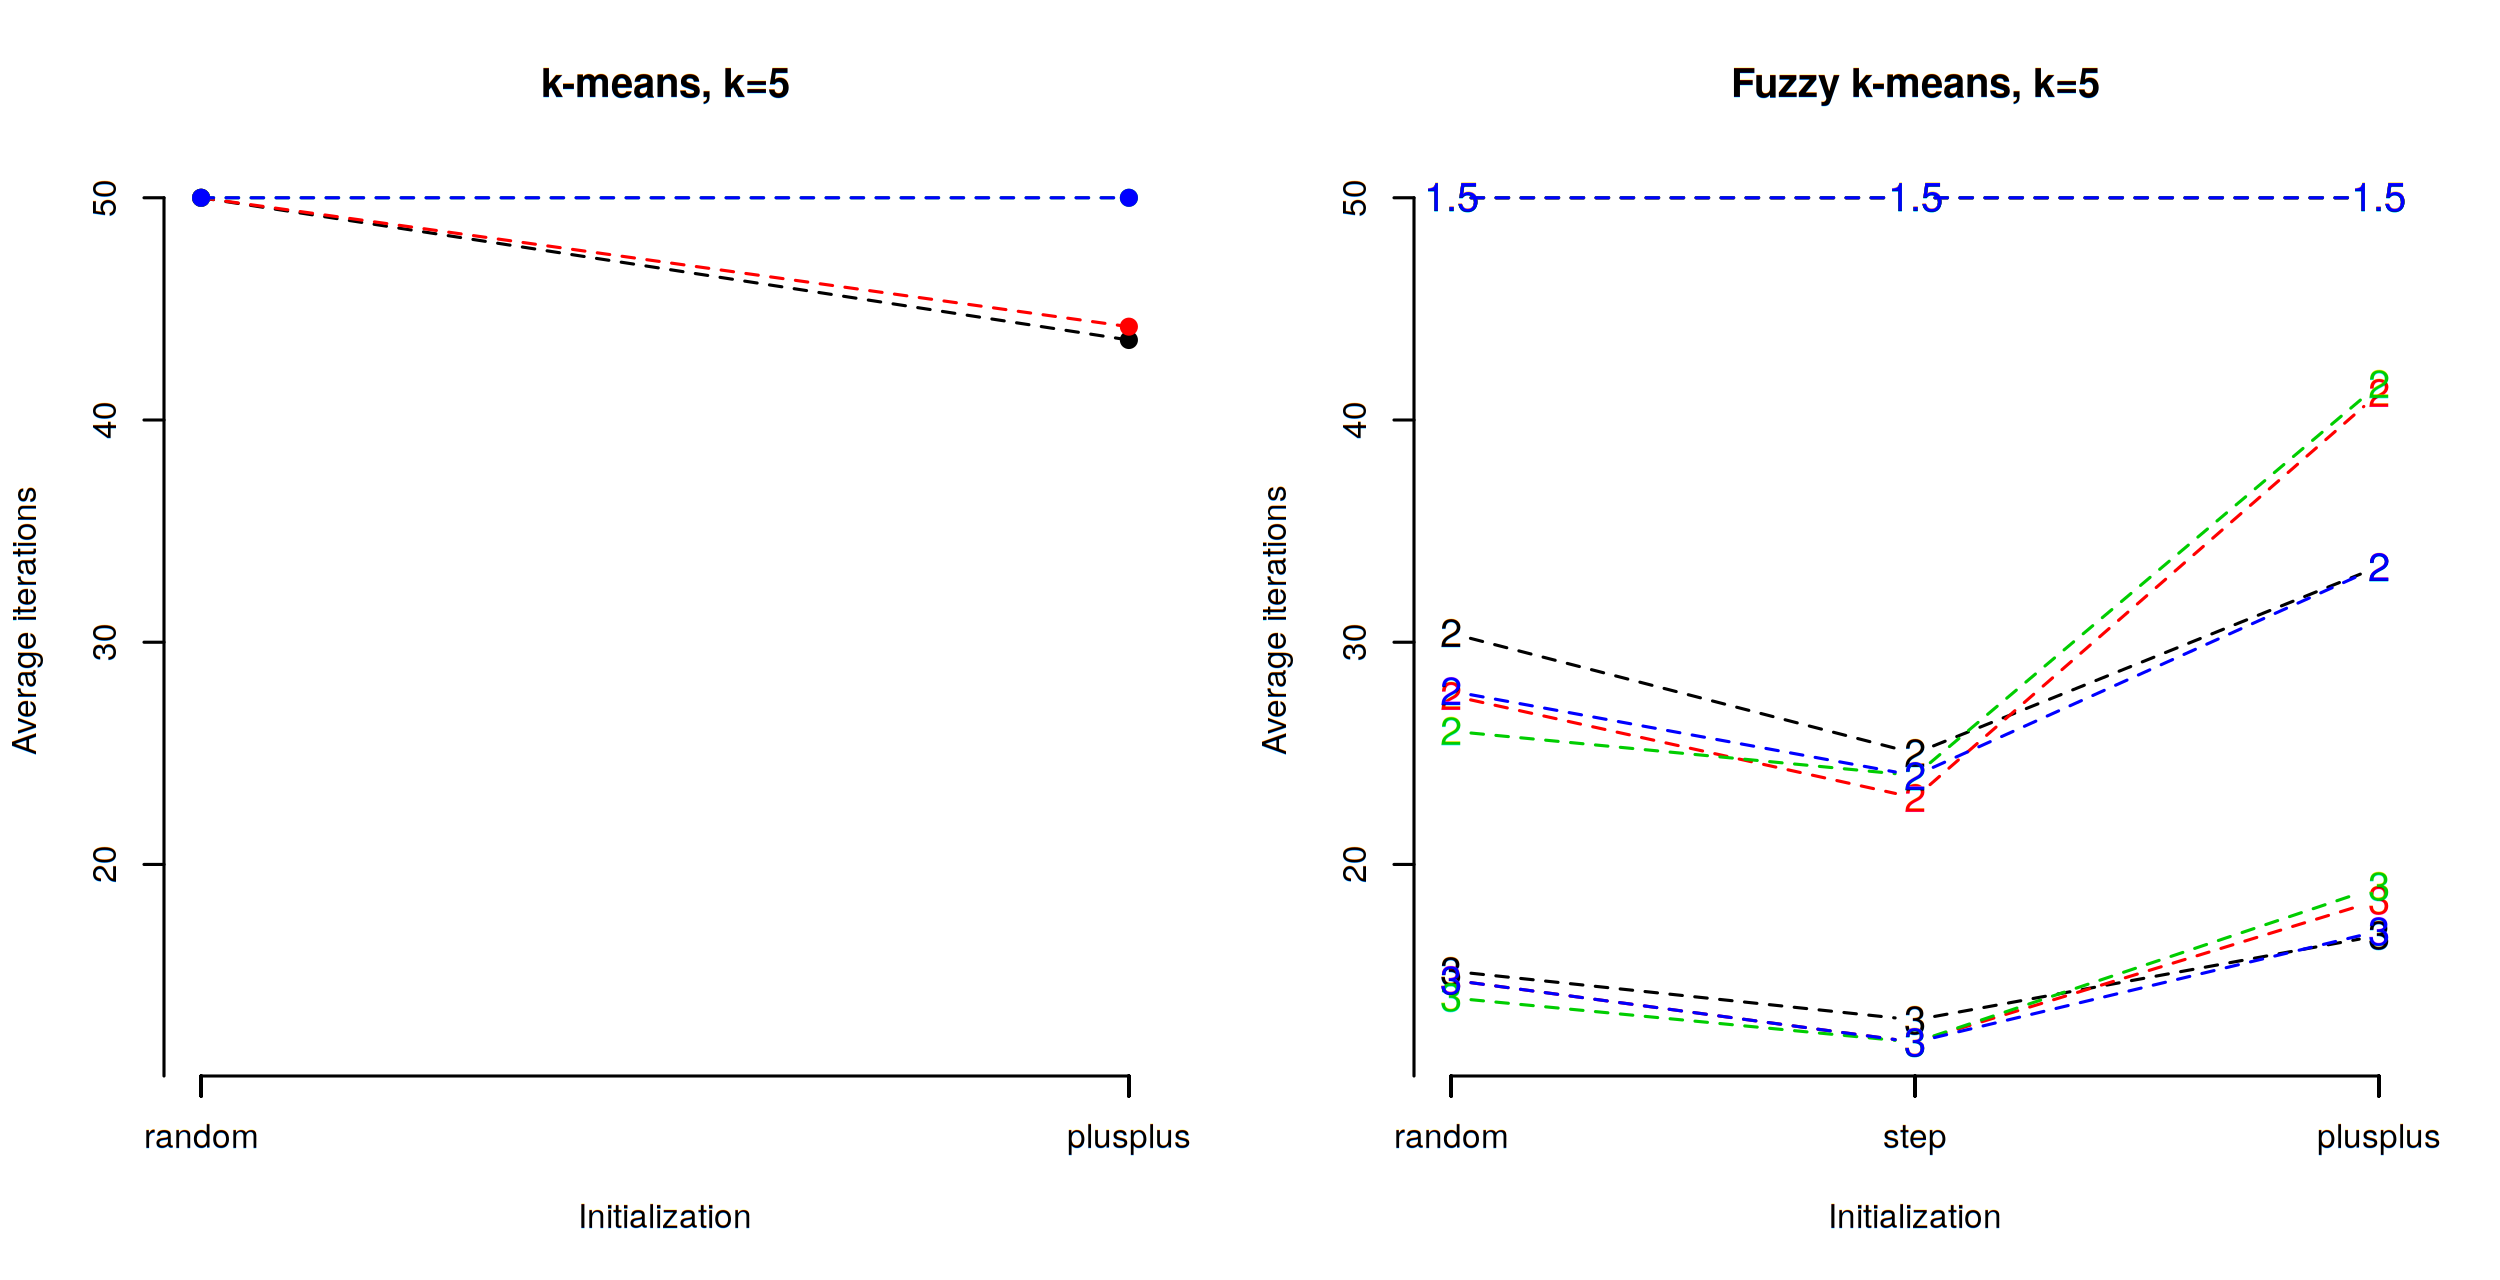
\includegraphics[width=0.94\textwidth]{figures/clust-5.png}
    \label{fig:results}
    \captionof{figure}{Prove empiriche sui dataset di dimensione 15000 (\textit{nero}), 30000 (\textit{rosso}), 70000 (\textit{verde}), 115473 (\textit{blu}). Per il \fcm\ sono riportati i diversi valori del parametro $m$ nel grafico.}
\end{center}

Nel caso del \km\ è stata omessa l'inizializzazione a step, in quanto soffre di una problematica non facilmente risolvibile: poiché i centroidi non vengono inizializzati scegliendo punti del dataset, alla prima iterazione può essere che non venga associata alcuna osservazione ad uno di essi. Di conseguenza, per costruzione degli algoritmi \mr, tale centroide viene eliminato e si ottiene un numero finale di centroidi minore di quanto specificato inizialmente. Per questo motivo, la procedura di inizializzazione a step è da evitare se si sceglie di utilizzare l'algoritmo \km. Nel caso dell'algoritmo \fcm, invece, questo problema non si presenta, in quanto l'aggiornamento della matrice di appartenenza e dei centroidi avviene in modo pesato sulla base della distanza.\\

Dai grafici, si osserva che l'inizializzazione ++ risulta vantaggiosa per il \km, portando mediamente a una riduzione del numero di iterazioni per $k=3$ e $k=5$, mentre per $k=4$ solo nel caso del dataset completo.
Nel caso del \fcm, si osserva che per tutti i valori di $k$, si ha un andamento molto simile dell numero di iterazioni al variare del grado di mescolamento $m$. L'inizializzazione a step, in questo caso, sembra portare a risultati migliori di convergenza dell'algoritmo.

%
% BibTeX users should specify bibliography style 'splncs04'.
% References will then be sorted and formatted in the correct style.
%
% {\color{red}\textbf{Descrivere dataset con variabili, dimensione,  ecc ecc}}\\
\bibliographystyle{splncs04}
\bibliography{progetto}
%

\begin{figure}
  \centering
  \subfigure[Daniele Zago]{
      % l b r t
  
\includegraphics[width=31mm,height=40mm]{figures/daniele-zago.png}}
  \subfigure[Giovanni Toto]{
  
\includegraphics[width=40mm,height=40mm]{figures/Giovanni_Toto.jpg}}
\end{figure}
\end{document}
